\documentclass[../Cours.tex]{subfiles}
\usepackage{multicol}
\usepackage[thicklines]{cancel}

\begin{document}

\setcounter{chapitre}{30}
\chapitre{Décomposition en facteurs premiers}
\partie{Primalité}
\souspartie{Nombres premiers}
\definition{Un nombre premier est un nombre qui n'est divisible que par lui-même ou par 1.}
\definition{Un nombre composé est un nombre qui n'est pas premier.}

\begin{listedexemples}
    \item 7 est un nombre premier. \\Il n'est pas possible d'écrire 7 sous la forme d'un produit de nombres entiers autre que $1 \times 7$. 
    \item 6 n'est pas un nombre premier car on peut écrire $6 = 3 \times 2$.
\end{listedexemples}

\souspartie{Critères de divisibilité}

\begin{center}
\begin{tabular}{|c|c|c|}\hline
     & Critère de divisibilité & Exemples  \\\hline
    Divisibilité par 2 & le nombre est pair & \makecell{\textcolor{vert}{8 est pair} \\ \textcolor{rouge}{7 est impair}}  \\\hline
    Divisibilité par 3 & la somme des chiffres est dans la table de 3 & \makecell{\textcolor{vert}{213 $\longrightarrow 2 + 1 + 3 = 6$} \\ \textcolor{vert}{6 est dans la table de 3} \\ \textcolor{rouge}{517 $\longrightarrow 5 + 1 + 7 = 13$} \\ \textcolor{rouge}{13 n'est pas dans la table de 3}} \\\hline
    Divisibilité par 5 & le chiffre des unités est 0 ou 5 & \makecell{\textcolor{vert}{315 : le chiffre des unités est 5} \\ \textcolor{rouge}{614 : le chiffre des unités est 4}} \\\hline
    Divisibilité par 9 & la somme des chiffres est dans la table de 9 & \makecell{\textcolor{vert}{216 $\longrightarrow 2 + 1 + 6 = 9$} \\ \textcolor{vert}{9 est dans la table de 9} \\ \textcolor{rouge}{517 $\longrightarrow 5 + 1 + 7 = 13$} \\ \textcolor{rouge}{13 n'est pas dans la table de 9}} \\\hline
    Divisibilité par 10 & le chiffre des unités est 0 & \makecell{\textcolor{vert}{310 : le chiffre des unités est 0} \\ \textcolor{rouge}{614 : le chiffre des unités est 4}} \\\hline
\end{tabular}
\end{center}

\partie{Théorème fondamental de l'arithmétique}
\souspartie{Énoncé du théorème}

\theoreme{}{N'importe quel nombre entier strictement positif peut être écrit \underline{de manière unique} comme un produit de nombres premiers.}

\begin{listedexemples}
    \item $234$ \\ $ = 2 \times 117$ \\ $ = 2 \times 9 \times 13$ \\ $ = 2 \times 3 \times 3 \times 13$
    \item $363$ \\ $ = 3 \times 121$ \\ $ = 3 \times 11 \times 11$
\end{listedexemples}


\souspartie{Application : simplification de fraction}

\methode{Pour simplifier le plus possible une fraction, on peut décomposer en facteurs premiers le numérateur et le dénominateur.}

\renewcommand{\CancelColor}{\color{rouge}}
\renewcommand{\labelitemii}{$\blacksquare$}
\begin{listedexemples}
\item Pour simplifier la fraction $\dfrac{39}{65}$ :
\begin{itemize}
\item Je décompose le numérateur : $39=3 \times 13$
\item Je décompose le dénominateur : $65=5 \times 13$
\item Donc $\dfrac{39}{65} = \dfrac{3 \times 13}{5 \times 13} = \dfrac{3 \times \cancel{13}}{5 \times \cancel{13}} = \dfrac{3}{5}$
\end{itemize}
\end{listedexemples}




\clearpage

\begin{questions}
    \exercice\\ Compléter le tableau suivant
    
    \begin{center}
    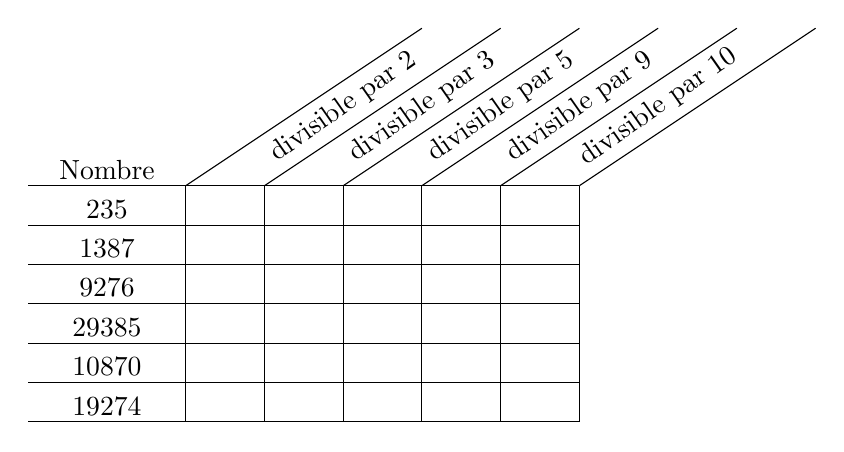
\begin{tikzpicture}
        \node at (1,0.2) {Nombre};
        \node at (1,-0.3) {235};
        \node at (1,-0.8) {1387};
        \node at (1,-1.3) {9276};
        \node at (1,-1.8) {29385};
        \node at (1,-2.3) {10870};
        \node at (1,-2.8) {19274};
        \foreach \y in {0,0.5,1,...,3} {
            \draw (0,-\y) -- (7,-\y);
        }
        \foreach \x in {2,3,...,7} {
            \draw (\x,0) -- (\x,-3);
            \draw (\x,0) -- (\x+3,2);
        }
        \node[rotate=35] at (4,1) {divisible par 2};
        \node[rotate=35] at (5,1) {divisible par 3};
        \node[rotate=35] at (6,1) {divisible par 5};
        \node[rotate=35] at (7,1) {divisible par 9};
        \node[rotate=35] at (8,1) {divisible par 10};
    \end{tikzpicture}
    \end{center}
    
    \exercice\\ Léa a décomposé le nombre 594 en produit de facteurs premiers. Elle a trouvé $594 = 2 \times 3 \times 9 \times 11$.
    \question Pourquoi son résultat n'est pas correct ?
    \question Donner la véritable décomposition en facteurs premiers de 594

    \exercice 
        \question Décomposer en facteurs premiers les nombres suivants
            \subpart 755
            \subpart 345
            \subpart 210
            \subpart 702
        \question Pour chacun des nombres de la 1ère question, donner tous leurs diviseurs
        
    \exercice\\ On dit qu'un nombre entier est parfait s'il est égal à la somme de tous ses diviseurs qui lui sont strictement inférieurs. Par exemple, les diviseurs de 6 sont : 1, 2, 3 et 6 (car $6 = 6 \times 1$ et $6 = 3 \times 2$). 6 est un nombre parfait car $1+2+3 = 6$.
        \question Vérifier que 28 est un nombre parfait
        \question Vérifier que 496 est un nombre parfait
        
        
    \exercice
        \question Décomposer en facteurs premiers les nombres suivants
        \vspace{-2ex}
        \begin{multicols}{4}
            \subpart 1275
            \subpart 765
            \subpart 306
            \subpart 510
        \end{multicols}
        \question Simplifier les fractions suivantes
        \vspace{-1ex}
        \begin{multicols}{5}
            \subpart $\dfrac{306}{510}$
            \subpart $\dfrac{765}{1275}$
            \subpart $\dfrac{306}{1275}$
            \subpart $\dfrac{1275}{510}$
            \subpart $\dfrac{765}{306}$
        \end{multicols}

\end{questions}


\end{document}